\documentclass[book.tex]{subfiles}
\begin{document}
\section{Programming}



Development was done with Borland C++ 3.1 (but the language used was C) which by default ran in EGA mode 3 offering a screen 80 characters wide and 25 characters tall.\\
\par
John Carmack took care of the runtime code. John Romero programmed many of the tools (TED5 map editor, IGRAB asset packer, MUSE sound packer). Jason Blochowiak wrote important subsystems of the game (Input manager, Sound manager, User manager).\\

\begin{figure}[H]
\centering
  \fullimage{compiling.png}
\caption{Borland C++ 3.1 editor}
\end{figure}
\par
Borland's solution was an all-in-one package. The IDE, \cw{BC.EXE}, despite some instabilities allowed crude multi-windows code editing with pleasant syntax highlights. The compiler and linker were also part of the package under \cw{BCC.EXE} and \cw{TLINK.EXE}\footnote{Source: Borland C++ 3.1 User Guide.}.
\pagebreak


There was no need to enter command-line mode however. The IDE allowed to create a project, build, run and debug.\\
\par
\begin{figure}[H]
\centering
  \fullimage{borland_compile.png}
  \caption{Compiling Keen Dreams with Borland C++ 3.1}
\end{figure}






Another way to improve screen real estate was to use "high resolution" 50x80 text mode.\\
\par 
 \fullimage{borland_ide_select.png}\\
 \par
 \vspace{-7pt}
The comments still fit perfectly on screen since only the vertical resolution is doubled.\\
\par
\vspace{-4pt}
 \fullimage{borland_ide_highres.png} 
 The file \cw{KD\_MAIN.C} opened in both modes demonstrates the readability/visibility trade-off.\\
\par

  \fullimage{borland_ide_main_lowres.png}\\
\vspace{-5pt}  
   %\vspace{-4pt}
\par
\vspace{5pt}
 \fullimage{borland_ide_main_highres.png}
\section{Graphic Assets}

All graphic assets were produced by Adrian Carmack. All of the work was done with Deluxe Paint (by Brent Iverson, Electronic Arts) and saved in ILBM\footnote{InterLeaved BitMap.} files (Deluxe Paint proprietary format). All assets were hand drawn with a mouse.

\begin{figure}[H]
  \centering
 \fullimage{deluxe_paint.png}
 \caption{Deluxe Paint was used to draw all assets in the game.}
\end{figure}


\subsection{Assets Workflow}
After the graphic assets were generated, a tool (IGRAB) packed all ILBMs together in an archive and generated a header table file (\cw{KDR}-format) and C header file with asset IDs. The engine references an asset directly by using these IDs.\\
\begin{figure}[H]
\centering
 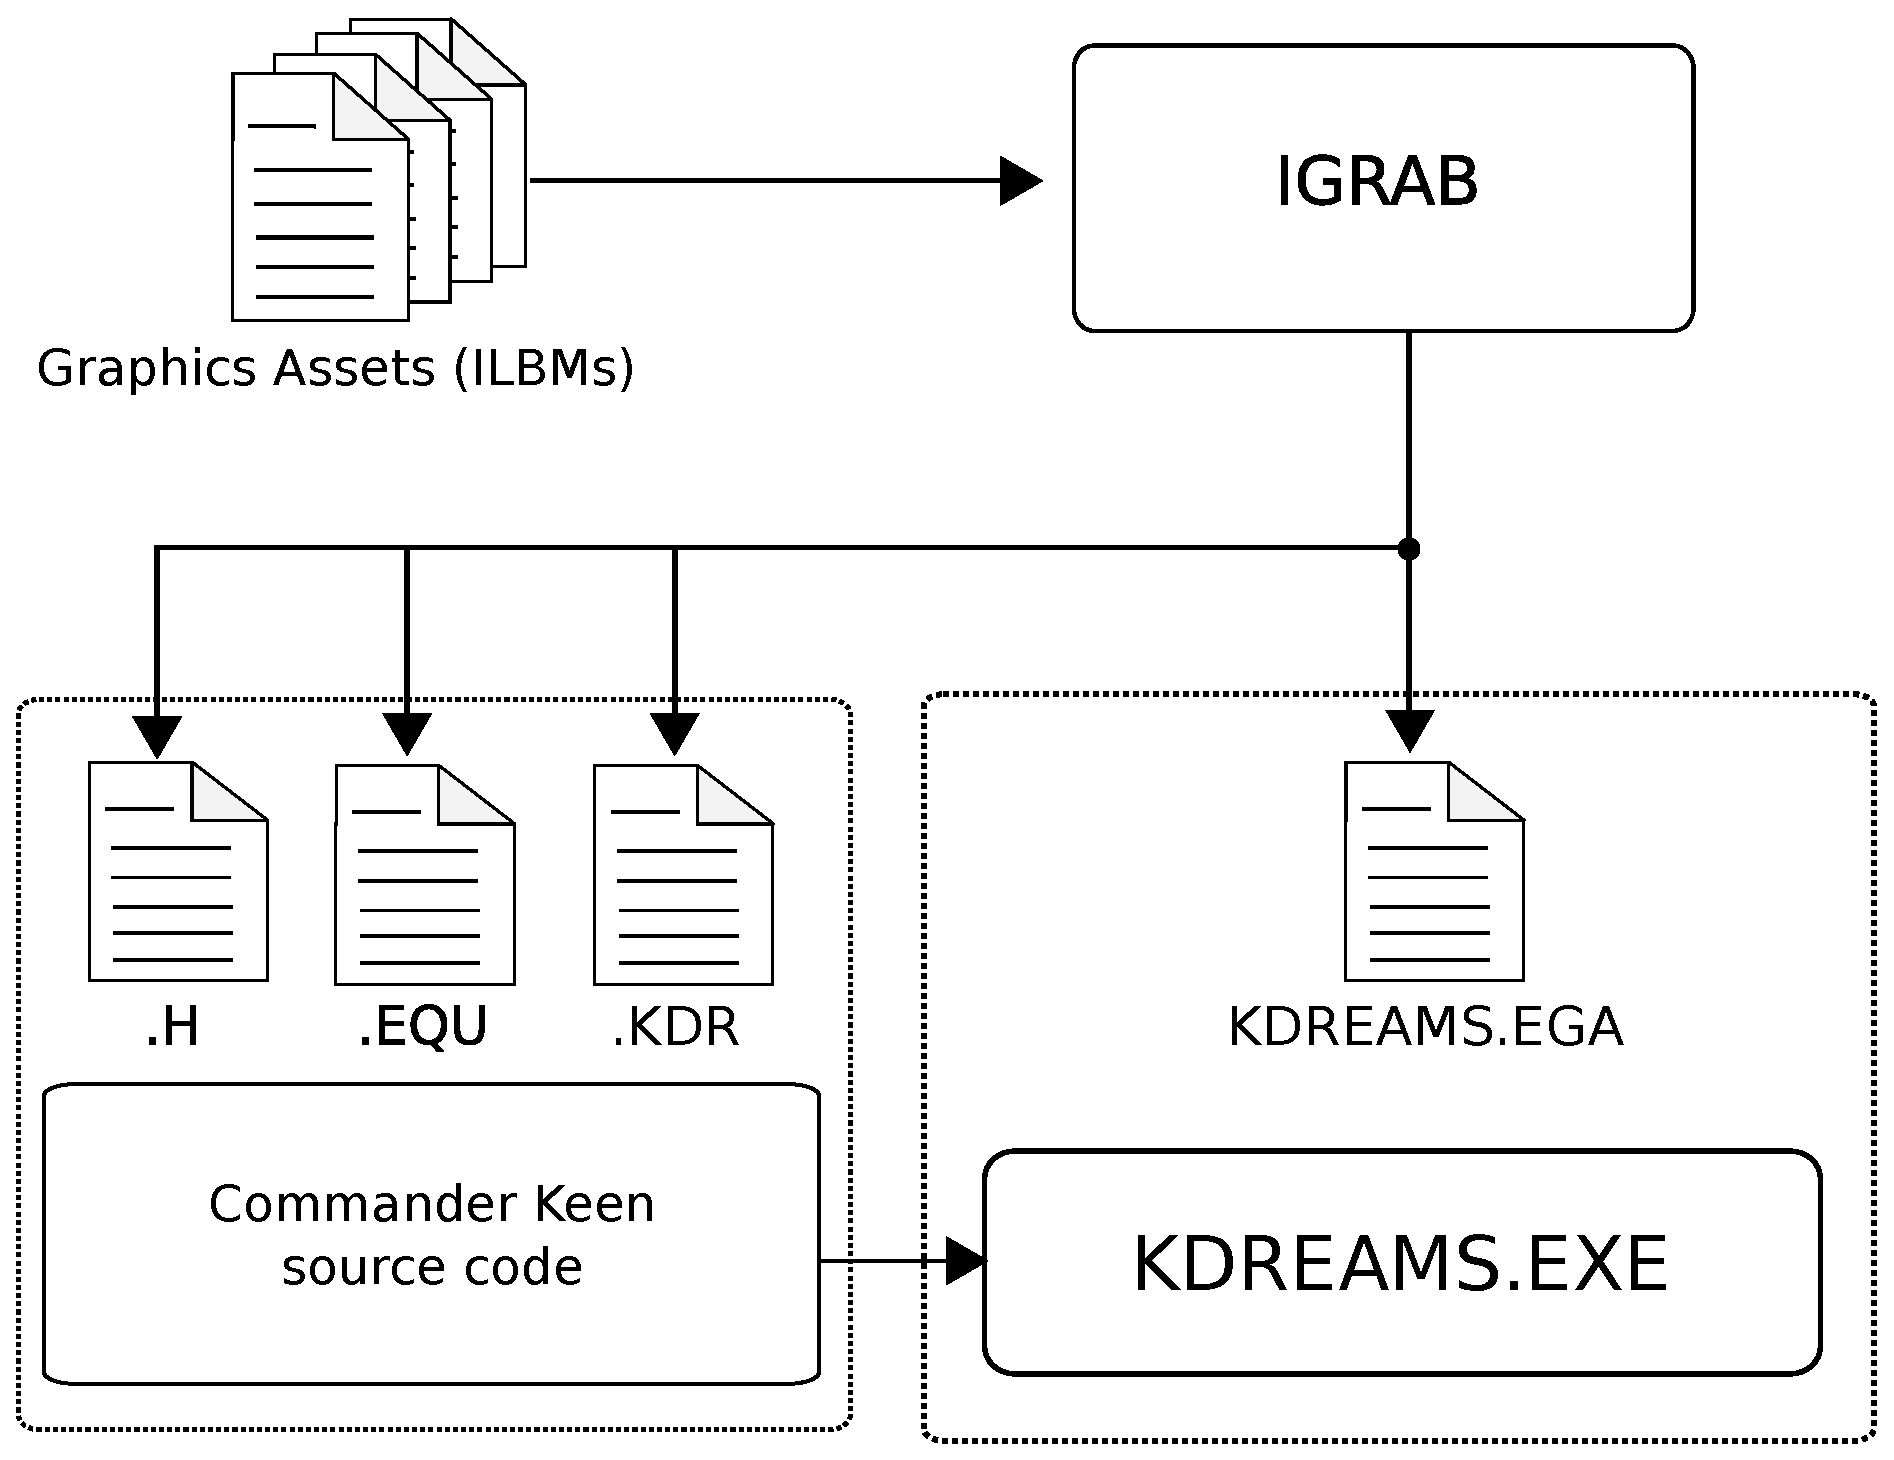
\includegraphics[width=.9\textwidth]{imgs/drawings/drawing_plain.eps}
 \caption{Asset creation pipeline for graphics items}
 \label{asset-creation-pipeline}
\end{figure}
\par
\begin{minipage}{\textwidth}
 \lstinputlisting[language=C]{code/assets_header.c}\par
 \end{minipage}
 
 In the engine code, asset usage is hardcoded via an enum. This enum is an offset into the \cw{HEAD} table which gives an offset in the \cw{DATA} archive. The \cw{HEAD} table files are stored in the \cw{\textbackslash static} folder as \cw{*.KDR} files.\\

\subsection{Assets file structure}
Figure \ref{fig:asset-creation-pipeline} shows the structure of the \cw{KDREAMS.EGA} asset file.
\begin{figure}[H]
\centering
 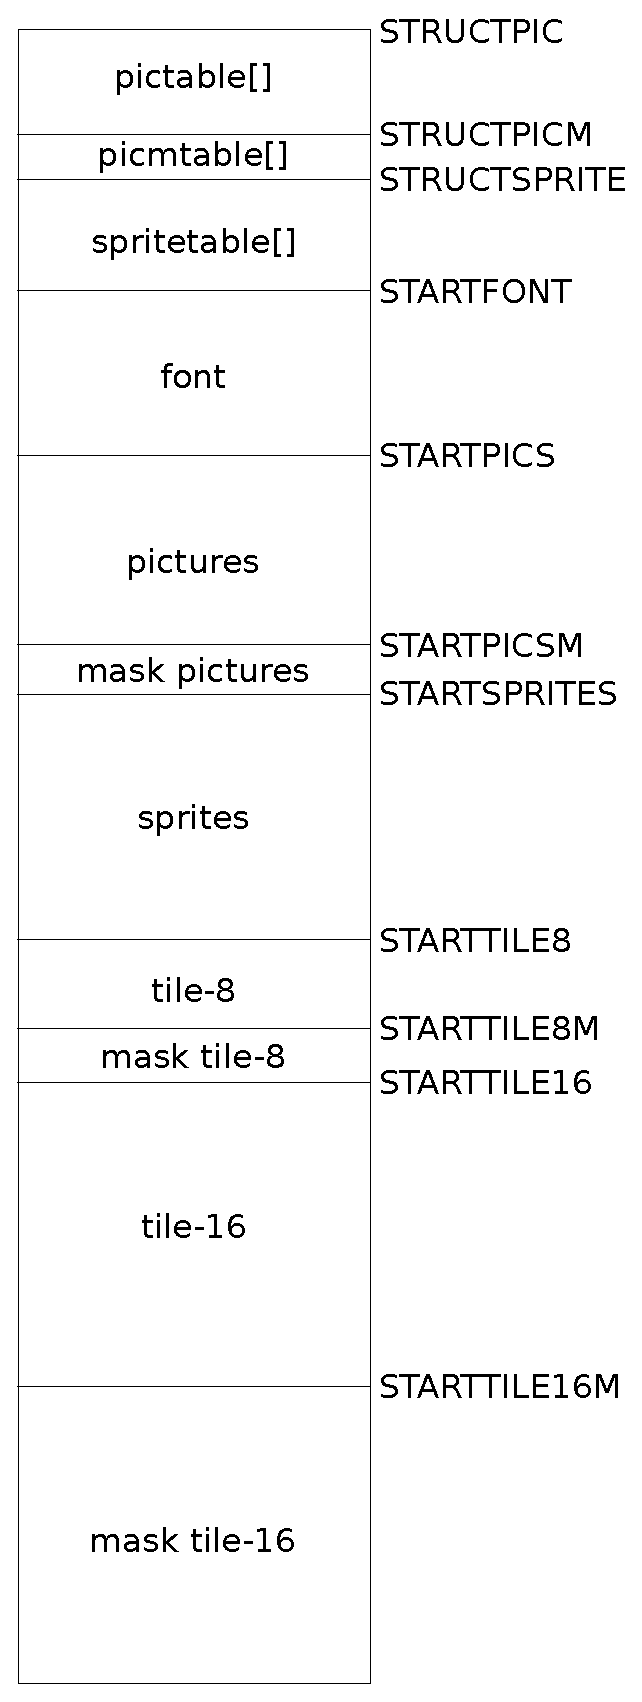
\includegraphics[width=.5\textwidth]{imgs/drawings/graphic_assets.eps}
 \caption{File structure of \cw{KDREAMS.EGA} asset file.}
 \label{fig:asset-creation-pipeline}
\end{figure}

The \cw{pictable[]} contains the width and height in bytes for each picture in the asset file. Note that a width of 5 bytes means a size of 40 pixels on the screen. The same size structure is applied for mask pictures.\\

  \begin{table}[H]
  \begin{tabularx}{0.8\textwidth}[c]{XXX}
  \hline
  \textbf{index} & \textbf{width} & \textbf{height}   \\ \hline
  0             & 5          & 32    \\
  1             & 5          & 32    \\
  2             & 5          & 32    \\
  3             & 5          & 32    \\
  4             & 5          & 32    \\
  5             & 5          & 32    \\
  6             & 5          & 32    \\
  7             & 5          & 32    \\
  ...             & ...          & ...    \\
  64             & 5          & 24    \\
  \end{tabularx}
  \caption{content of pictable[].}
  \end{table}



The \cw{spritetable[]} contains beside width and height in bytes also information on the sprite center, hit boundaries and number of shifted sprites (this will be explained in section xxx). \\

\begin{table}[H]
  \begin{tabularx}{\textwidth}[c]{lXXXXXXXXX}
  \hline
  \textbf{index} & \textbf{width} & \textbf{height} & \textbf{orgx} & \textbf{orgy}
    & \textbf{xl} & \textbf{yl} & \textbf{xh} & \textbf{yh} & \textbf{shift} \\ \hline
  0  &   3  &   24  &   0  &   0  &   0  &   0  &   368  &   368  &   4 \\
  1  &   3  &   32  &   0  &   0  &   64  &   0  &   304  &   496  &   4 \\
  2  &   3  &   30  &   0  &   16  &   64  &   0  &   304  &   496  &   4 \\
  3  &   3  &   30  &   0  &   32  &   64  &   48  &   304  &   496  &   4 \\
  4  &   3  &   32  &   0  &   0  &   64  &   0  &   304  &   496  &   4 \\
  5  &   3  &   30  &   0  &   32  &   64  &   48  &   304  &   496  &   4 \\
 ...  &   ...  &   ...  &   ...  &   ...  &   ...  &   ...  &   ...  &   ...  &   ... \\
 296  &   12  &   103  &   -128  &   0  &   256  &   128  &   752  &   1648  &   4\\
  \end{tabularx}
  \caption{content of spritetable[].}
  \end{table}

As all tiles have fixed dimension (either 8 or 16 pixels), there is no need to store any tile size table structure. From \cw{STARTPICS} location onwards all assets are stored.
 
\begin{figure}[H] 
  \centering 
  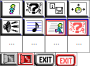
\includegraphics[width=1.0\textwidth, frame]{screenshots_300dpi/pics_assets.png}
  \caption{Picture assets data.}
  \label{fig:picture_assets}
\end{figure} 

\begin{figure}[H] 
  \centering 
  \includegraphics[width=1.0\textwidth, frame]{screenshots_300dpi/sprite_assets.png}
  \caption{Sprite assets data.}
  \label{fig:sprite_assets}
\end{figure} 

\begin{figure}[H] 
  \centering 
  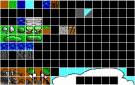
\includegraphics[width=0.9\textwidth, frame]{screenshots_300dpi/tile16_assets.png}
\end{figure} 

\begin{figure}[H] 
  \centering 
  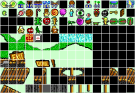
\includegraphics[width=0.9\textwidth, frame]{screenshots_300dpi/tile16M_assets.png}
  \caption{Tile-16 and masked tile-16 assets data.}
  \label{fig:tile16_assets}
\end{figure} 



\section{Maps}
Maps were created using an in-house editor called TED5, short for Tile EDitor. TED5 was not created specially for Wolf 3D, but was originally made for the Commander Keen series and improved over the years. It was a versatile tool since it allowed for creating maps of both side-scroller games and top-down games like Rescue Rover and Wolf 3D.\\
\par
 TED5 is not stand-alone; in order to start, it needs an asset archive and the  associated header (as described in the graphic asset workflow Figure \ref{asset-creation-pipeline} on page \pageref{asset-creation-pipeline}). This way, texture IDs are directly encoded in the map.\\

 
 \fullimage{TedSplashscreen.png}
 \par
 \trivia{The suffix, "vD.IP", was put in by the Rise of the Triad team in 1994. It stood for "Developers of Incredible Power".}\\
 \par
\fullimage{Fill_2.png}\\
 


 \fullimage{ted5_scrolling_map.png}\\
\par
\vspace{20pt}
\par
 \fullimage{TED.png}


 \par
 TED5 allows placement of tiles on layers called "planes". This layered approach proved powerful and versatile. In Commander Keen, layers are used for background, tiles which the hero can stand on, generating bonuses and so on. For Wolfenstein 3D, two layers are used: one for walls, and one to place bonuses and enemies on.\\
 \par

Reusing TED5 was a double win. Not only did it save tool development time, but ramp-up time was also reduced as all team members had been using it for years. TED5 was so good at doing the job that it allowed designers to make a level within minutes\footnote{TED5 was used in 33 commercially shipped games (including Rise of the Triad in 1994).}.\\
\par

 \begin{fancyquotes}
After talking with Romero and Tom, Scott learned that it was taking the group only about one day to make a level of the game. Ka-chung! Dollar signs! Instead of just three episodes, why not have six? Scott said, "If you can do thirty more levels, it would only take you fifteen days. And we could have it where people could buy the first trilogy for thirty-five dollars or get all six for fifty dollars, or if people buy the first episode and later want the second episodes it will be twenty dollars. So there's a reason to get them all!" After some consideration, id agreed.\\
\\
 \textbf{- Masters of Doom}
 \end{fancyquotes}\\

\par
John Romero and Tom Hall did all the map design with TED5. Bobby Prince helped too and is credited for maps E6M2 and E6M3.\\
\par
 \textbf{\underline{Trivia :}} The source code of TED5 was released several years later. Among the source code made of \cw{.C} and \cw{.H} was a mysterious \codeword{\_TOM.PIC}\footnote{Intentionally not reproduced here.}. It turned out to be an adult caricature of Tom Hall made by Adrian Carmack. The explanation came from John Romero:\\% in 2002:\\
\par
 \begin{fancyquotes}
   "Hahahaha! Wow, I forgot all about that picture. I can't believe it's 
in the TED5 source files! It's basically a pic that Adrian drew of Tom 
[...] saying "Sorry!".\\
\par 
It's because Tom and Adrian used to share a worktable together. Tom 
would always bump the table while Adrian was drawing graphics with the 
mouse and Tom would say, "Sorry!".\\
   \\
\textbf{John Romero - Programmer}
 \end{fancyquotes}


\end{document}
